\twocolumn[
	\section{Solution}\label{ch:solution}
	]
	
%	In essence, the challenge is how to correlate the on-screen input space with the data retrieved from the tracking device. 
%: initiating swiping on-screen and veering off-screen while maintaining a fluent sense of continuous input and precision.	
\noi
Here, the theoretical foundation of the solution is outlined in three steps. The first step involves finding the correlation between on-screen and off-screen space, which will  allow for converting any motion tracking point to an equivalent position in the information space. Such translation obviously depends on the definition of off-screen space, i.e. the shape of the imaginary extension of the display plane. This constitutes the second task, defining potential shapes of the off-screen space. Finally, in order to align with the goals of the solution it will be necessary to ensure that the transition between the two spaces is smooth and appears close to transparent to the user. 
%That is, the going from on-screen input and to the translated position, facilitated by the definition of off-screen space.

\newcommand\plotClass[3]{
	\addplot[ scatter, point meta=explicit symbolic, discard if not={label}{#1}, color=#2,
	scatter/classes={
		#1={#3,mark=*,mark size=3pt}
	},
	] table[meta=label] {data/projection.csv} 
}


Overall, the most challenging task was found to be the first of the three, i.e. determining the exact location, orientation and scale of the on-screen space in off-screen space. The remaining two tasks were simpler and more isolated by nature, as well more comprehensible because they had incremental effects that could easily be visualized.\\

\subsection{Correlating spaces}

We will refer to the correlating of on-screen and off-screen space as the \ti{calibration} portion of the solution. This may be broken down into well-defined sub-steps. First, the dimensions of the on-screen space (which takes the shape of a rectangle) is defined. This is required because only a portion of the Surface screen is used (for emulating a smaller display). Next, a close approximation of the spatial  (off-screen) location, scale and orientation of this rectangle is determined through tracking data. Lastly, the approximation is adjusted to compensate for minor deviations between the side ratios of the two (tracking noise being one cause of this). The end result is then two identically shaped but differently sized rectangles, which implicitly give the scaling ratio between the on-screen and off-screen space.

\subsubsection{On-screen input space}

Our initial subtask is to derive the rectangle that represents the on-screen input space. The lines of this rectangle then marks the transition boundaries into off-screen space. Put differently, when the user initiates a swipe on-screen and moves beyond these transition lines, he or she will be navigating in the off-screen space. Furthermore, we would like this rectangle to have lines running parallel with the device form factor. 

To achieve this, data points for the boundaries are collected by having the user run the index finger along the lines on the input space in a single operation, after which the input is processed. Naturally, manual input is unlikely to produce a perfect rectangle, nor have lines that run perfectly parallel with the form factor of the display. To overcome this, a fitting equal to maximizing a rectangle within these boundaries will be assumed preferable. An exaggerated example is shown in figure \ref{fig:2dRectFit}. %We note that the "disregarded" areas are assumed to be small, negligible and mostly of relevance to the implementation logic.

\begin{figure}[!h]
	\begin{center}
		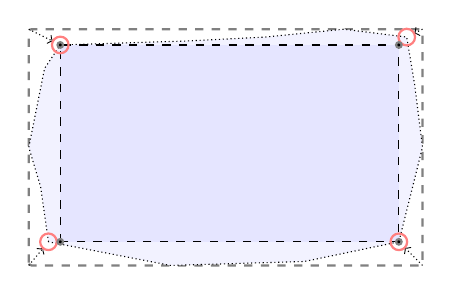
\begin{tikzpicture}[scale=1]
		
		%		
		\coordinate (P1) at (0,0);
		\coordinate (P2) at (0,3);
		\coordinate (P3) at (5,3);
		\coordinate (P4) at (5,0);
		
		\coordinate (C1) at (0.25,0.3);
		\coordinate (C2) at (0.4,2.8);
		\coordinate (C3) at (4.8,2.9);
		\coordinate (C4) at (4.7,0.3);
		
		
		\draw[thick,dashed,rounded corners = 1pt, gray] (P1) -- (P2) -- (P3) -- (P4) -- (P1) -- cycle;
		
		% L,T,R,B
		\draw[densely dotted, fill=blue!5] 
		(0.25,0.3) -- (0.15,1) --  (0,1.5) -- (0.2,2.5) -- (0.4,2.8) -- 
		(2,2.85)  -- (3,2.9) -- (4,3) -- (4.8,2.9) -- (4.9,2.3) --  (5,1.5) -- 
		(4.7,0.3) -- (3.5,0.05) -- (1.8,0) -- 
		cycle;
		
		\draw[->,densely dotted,black,shorten >=.1cm] (P1) -- (C1);
		\draw[->,densely dotted,black,shorten >=.1cm] (P2) -- (C2);
		\draw[->,densely dotted,black,shorten >=.1cm] (P3) -- (C3);
		\draw[->,densely dotted,black,shorten >=.1cm] (P4) -- (C4);
		
		
		% the inner rect
		\def\innerRect{
			(0.4,0.3) -- (0.4,2.8)  -- (4.7,2.8) -- (4.7,0.3) -- cycle
		}
		%		\draw[thick,dashed,rounded corners = 1pt, gray] \innerRect;
		%		\runeshade{dashed}{blue!10}{white} \innerRect;
		\draw[dashed, fill=blue!10] \innerRect;
		
		
		\draw[thick, color=red!50](C1) circle[radius = 3pt];
		\draw[thick, color=red!50](C2) circle[radius = 3pt];
		\draw[thick, color=red!50](C3) circle[radius = 3pt];
		\draw[thick, color=red!50](C4) circle[radius = 3pt];
		%
		\draw[thick, color=black!50, fill=black](0.4,0.3) circle[radius = 1pt];
		\draw[thick, color=black!50, fill=black](0.4,2.8) circle[radius = 1pt];
		\draw[thick, color=black!50, fill=black](4.7,2.8) circle[radius = 1pt];
		\draw[thick, color=black!50, fill=black](4.7,0.3) circle[radius = 1pt];
		%
		
		\end{tikzpicture}
		\caption{\small Fitting the input space: from the maximum device-aligned rectangle span of the input points (outer rectangle), inner rectangle corner candidates are identified (red circles) and the final fit (inner rectangle) equals the maximization of a rectangle within the space spanned by these candidates.}
		\label{fig:2dRectFit}
	\end{center}
\end{figure}

%Each corner of this rectangle will be  "ideal" in the sense that they would be true representations of the input space corners, were it not for the expected crooked corners. 
To produce this rectangle fit, the maximum top, right, bottom and left components are first identified from the full set of input points. This initially identifies both the location and the maximum possible dimensions of the input, corresponding to the outer rectangle in figure \ref{fig:2dRectFit}. To reach the desired smaller fit, a more appropriate set of corners is identified by, for each corner, picking the nearest neighbor from the full set of input points, i.e. the input point with shortest distance. The input space is then defined by the maximization of a rectangle within the space spanned by these new corner points. 
%To ensure a proper callibration, the end result is presented to the user as a transparent overlay that allows for easy visual verification, as shown in figure ??????.

We note that the orientation of this fitted rectangle is implicit. That is, the rectangle has sides top, bottom, left and right, as seen from the viewpoint of the user that provided the input. We will adopt these names to describe orientations, which will be relevant later on.


\subsubsection{Off-screen input plane}

The derivation of the device plane in off-screen space will be performed by the fitting of a set of spatial points, each assumed to be in close proximity to the plane spanned by the device. These points are in fact already available to us: in the previous derivation of the on-screen rectangle, pairings between on-screen and off-screen points were done. Hence, the fitting data is implicitly available as a set of  spatial tracking data points that should align closely with some plane (again, not perfectly due to factors such as tracking noise).% and the spatial corners of the on-screen plane.

%\fn{Technically each pairing instantiated at the availability of a new tracking point with the most recent on-screen input location. This makes each pairing unique, because the tracking device is the limiting factor (due the lower frame ratio of approximately 20 to 30 frames per second.)}. 
 
\paragraph{Geometrical view of the fitting}

To fit a plane to the set of spatial points, we will approach this as an optimization problem with some error to minimize. An intuitive choice would be attempting to express the sum of all projection distances to the plane of choice and then use calculus to differentiate and solve for the minimum. However, this would involve calculating Euclidean distances in multi-dimensional space, which cannot easily be differentiated. 

To identify an alternative fitting strategy, we will give some thought to the geometry of the tracking points. In particular, if we assume that the tracking noise is Gaussian with the mean spanning a plane, we get geometry such as  that shown in figure \ref{fig:fitSinePlane}. 

%The first step in processing this set of spatial data points is to derive some plane by which they are assumed to fluctuate around, as illustrated in figure \ref{fig:fitSinePlane}. This task is challenged by the degree of inherent imprecision in the spatial tracking mechanism, a factor that is expected to be present but minimal. 

\begin{figure}[!h]
	\begin{center}	
		\begin{tikzpicture}[x={(290:0.8cm)}, y={(-10:1cm)}, z={(0,1cm)}, scale=1.2,
		%		\begin{tikzpicture}[x={(-160:1cm)}, y={(-20:1cm)}, z={(0,1cm)}, scale=1.2,
		%		\begin{tikzpicture}[x={(-180:1cm)}, y={(180:0.8cm)}, z={(0,1cm)}, scale=1.2,
		plane max z=3]
		
		\node[text width=0.2cm,gray] at (4,-0.3,0) {\small x};
		\node[text width=0.2cm,gray] at (-0.3,4,0) {\small y};
		\node[text width=0.2cm,gray] at (0,-0.25,4) {\small z};
		
		\draw[->] (0,0,0) -- (4,0,0);
		\draw[->] (0,0,0) -- (0,4,0);
		\draw[->] (0,0,0) -- (0,0,4);
		
		\definePlaneByEquation{myplane}{1}{1}{1}{3}
		\drawPlane[thick,fill=blue!4]{myplane}
		
		\begin{loopTabbedCsv}[data/sinePlaneFitPoints.csv]{sinePlaneFitPoints}{\x=x,\y=y,\z=z}
		\definePointByXYZ{p51}{\x}{\y}{\z};
		\draw[color=red!50](p51) circle[radius = 1pt];
		\projectPointToPlane{projp51}{p51}{myplane}
		\fill[color=black!80](projp51) circle [radius=1pt];
		\draw[->, shorten <= 1pt, shorten >= 1pt, color = gray!60](p51) -- (projp51);
		\end{loopTabbedCsv}
		
		
		\end{tikzpicture}
		\caption{A sequence of spatial points, generated by departing a sine curve along the the normal of the easily comprehensible example plane  $x + y + z = 3$. The departure magnitude is defined by sampling from a Gaussian distribution with zero mean. Given a set of these points, this plane could therefore be considered an appropriate fitting.}
		\label{fig:fitSinePlane}
	\end{center}
\end{figure}





Additional insight is obtained when viewing this example in profile, as shown in figure \ref{fig:fitSinePlane2}. From this, we see that with Gaussian noise we will see equal fluctuations  on either side of the plane fit. In addition, choosing to project along a single axis should not change the plane fit, since the result is merely a scaling of the projection lengths, as illustrated in figure \ref{fig:fitSinePlaneAlongZ}. The geometric relations of this observation are further illuminated in figure  \ref{fig:axisProjectionIsTriangle}, which shows that this approach scales each plane-orthogonal projection length by the inverse of the angle between the plane's normal and the projection axis (i.e. a constant factor).




\begin{figure}[!h]
	\begin{center}	
		%		\begin{tikzpicture}[x={(290:0.8cm)}, y={(-10:1cm)}, z={(0,1cm)}, scale=1.2,
		%		\begin{tikzpicture}[x={(-160:1cm)}, y={(-20:1cm)}, z={(0,1cm)}, scale=1.2,
		\begin{tikzpicture}[x={(-180:1cm)}, y={(180:0.8cm)}, z={(0,1cm)}, scale=1.2,
		plane max z=3]
		%		\node[text width=0.2cm,gray] at (4,-0.3,0) {\small x};
		%		\node[text width=0.2cm,gray] at (-0.3,4,0) {\small y};
		\node[text width=0.2cm,gray] at (0,-0.25,4) {\small z};
		
		\draw[->] (0,0,0) -- (4,0,0);
		\draw[->] (0,0,0) -- (0,4,0);
		\draw[->] (0,0,0) -- (0,0,4);
		
		
		
		\definePlaneByEquation{myplane}{1}{1}{1}{3}
		\drawPlane[thick,fill=blue!4]{myplane}
		
		%		\input{data/sinePlaneFitPoints}
		
%\csvloop{
%	file=data/sinePlaneFitPoints.csv,
%%	no head,
%	head to column names,
%	command={
%			\definePointByXYZ{p51}{\x}{\y}{\z};
%			\draw[color=red!50](p51) circle[radius = 1pt];
%			\projectPointToPlane{projp51}{p51}{myplane}
%			\fill[color=black!80](projp51) circle [radius=1pt];
%			\draw[->, shorten <= 1pt, shorten >= 1pt, color = gray!60](p51) -- (projp51);
%	},
%	late after line=,
%	late after last line=,
%}		

		\begin{loopTabbedCsv}[data/sinePlaneFitPoints.csv]{sinePlaneFitPoints}{\x=x,\y=y,\z=z}
			\definePointByXYZ{p51}{\x}{\y}{\z};
			\draw[color=red!50](p51) circle[radius = 1pt];
			\projectPointToPlane{projp51}{p51}{myplane}
			\fill[color=black!80](projp51) circle [radius=1pt];
			\draw[->, shorten <= 1pt, shorten >= 1pt, color = gray!60](p51) -- (projp51);
		\end{loopTabbedCsv}
		
		
		
		\end{tikzpicture}
		\caption{A profile view of the example plane with orthogonal projections.}
		\label{fig:fitSinePlane2}
	\end{center}
\end{figure}

\begin{figure}[!h]
	\begin{center}	
		%		\begin{tikzpicture}[x={(290:0.8cm)}, y={(-10:1cm)}, z={(0,1cm)}, scale=1.2,
		%		\begin{tikzpicture}[x={(-160:1cm)}, y={(-20:1cm)}, z={(0,1cm)}, scale=1.2,
		\begin{tikzpicture}[x={(-180:1cm)}, y={(180:0.8cm)}, z={(0,1cm)}, scale=1.2,
		plane max z=3]
		%		\node[text width=0.2cm,gray] at (4,-0.3,0) {\small x};
		%		\node[text width=0.2cm,gray] at (-0.3,4,0) {\small y};
		\node[text width=0.2cm,gray] at (0,-0.25,4) {\small z};
		
		\draw[->] (0,0,0) -- (4,0,0);
		\draw[->] (0,0,0) -- (0,4,0);
		\draw[->] (0,0,0) -- (0,0,4);
		
		\definePlaneByEquation{myplane}{1}{1}{1}{3}
		\drawPlane[thick,fill=blue!4]{myplane}
		
		%		\input{data/sinePlaneFitPointsAlongZ}
		
		\begin{loopTabbedCsv}[data/sinePlaneFitPoints.csv]{sinePlaneFitPoints}{\x=x,\y=y,\z=z}
		\definePointByXYZ{p51}{\x}{\y}{\z};
		\draw[color=red!50](p51) circle[radius = 1pt];
		\projectPointToPlaneAlongZ{projp51}{p51}{myplane}
		\fill[color=black!80](projp51) circle [radius=1pt];
		\draw[->, shorten <= 1pt, shorten >= 1pt, color = gray!60](p51) -- (projp51);
		
		\projectPointToPlane{projp51}{p51}{myplane}
		\fill[color=black!80](projp51) circle [radius=1pt];
		\draw[->, dotted, shorten <= 1pt, shorten >= 1pt, color = gray](p51) -- (projp51);
		\end{loopTabbedCsv}
		
		
		\end{tikzpicture}
		\caption{Projecting points to the plane along the z-axis, with previously shown projections normal to the plane shown as dotted lines. With a 45 degree plane, each projection length is now $\i1/{sin (45\degree)} = \sqrt{2}$ that of the orthogonal projection. While the z-aligned projections obviously obfuscate the original sine curve, the plane fitting remains unaffected, which is our sole interest.}
		\label{fig:fitSinePlaneAlongZ}
	\end{center}
\end{figure}

\begin{figure}[!h]
	\begin{center}
		\begin{tikzpicture}
		
		
		%	\draw[->] (0,0,0) -- (4,0,0);
		%	\draw[->] (0,0,0) -- (0,4,0);
		%	\draw[->] (0,0,0) -- (0,0,4);
		%	
		%	\definePlaneByEquation{myplane}{1}{1}{1}{3}
		%	\drawPlane[thick,fill=blue!4]{myplane}
		
		%	\drawPlane[thick,fill=blue!4]{myplane}
		
		%	\newcommand{\pOne}{(0,2)}
		
		\begin{scope}[rotate=63.4
		]
		
		\coordinate (P1) at (0,0);
		\coordinate (P2) at (-4,0);
		\coordinate (P23) at (-2, 2);
		\coordinate (P3) at (0,2);
		
		\coordinate (U) at (2,1);				
		
		\coordinate (U1) at (0,0.5);				
		\coordinate (U2) at (-0.5,0.5);				
		\coordinate (U3) at (-0.5,0);				
		
		
		\begin{scope}[shift={(-0.8,2)}]
		
		\coordinate (Q1) at (0,0);
		\coordinate (Q2) at (-4,0);
		\coordinate (Q3) at (0,2);
		
		%					\shade[top color=blue!13!white,opacity=0.5] (-1,0) (P1) -- (P2) -- (Q2) -- (Q1) -- cycle;
		
		%				\IFBUILDSTART
		%				\shade[top color=blue!13!white,opacity=0.5] (P1) -- (P2) -- (P3) -- cycle;
		%				\IFBUILDEND			
		%					
		\end{scope}
		
		
		\drawWithBuildOption{white}{top color=\themeColorLight} (P1) -- (P2) -- (P3) -- cycle;
%		\draw[white,top color=\themeColorLight] (P1) -- (P2) -- (P3) -- cycle;
		
		\pic [thick, draw, ->, "$\theta$", angle eccentricity=1.7] {angle = P1--P2--P3};
		
		\draw[->,thick,dashed,rounded corners = 1pt, gray] (P1) -- (U);
		
		\draw[thick,rounded corners = 1pt, black] (P1) -- (P2);
		
		\draw[very thick,dashed,gray] (P1) -- (Q1) -- (Q2) -- (P2);
		
		\draw[thick,gray] (U1) -- (U2) -- (U3);
		
		%				\draw[->,very thick,black] (P2) -- (P23);
		\draw[->,very thick,black,shorten >=.1cm] (P3) -- (P2);
		\draw[->,very thick,black,shorten >=.1cm] (P3) -- (P1);
		
		\draw[very thick, color=red!50](P3) circle[radius = 3pt];
		
		\end{scope}
		
		\node[text width=0.4cm,gray, rotate=87,yslant=-0.5] at (-3.87,-1.9) {plane};
		
		\node[text width=0.2cm,gray!70] at (0.4,1.5) {$\b{u}$};
		\node[text width=0.3cm,black] at (-1,0.9) {$ - p \ \b{\hat{n}}$};
		%			\node[text width=0.2cm,black] at (-1.3,2) {$$};
		\node[text width=0.2cm,black] at (-0.5,-1.8) {$b$};
		\node[text width=0.4cm,black] at (-2.6,-1.8) {$ - h \  \b{\hat{u}}$};
		%			\node[text width=0.2cm,black] at (-3.2,1.8) {$h$};
		%			\node[text width=0.2cm,black] at (-3.2,-1.3) {$\hat{k}$};
		
		\end{tikzpicture}
		\caption{A closer examination of the alternative (axis-aligned) projection: given plane-orthogonal projection length $p$, the alternative axis-aligned projection length $h$ will be equal to the hypotenuse of the right triangle formed by $p$ and the planar distance $b$ between the two projections. Hence,  $ h= \ifrac{p}{\sin\theta} $ (since $\sin \theta = \i{p}/h$), which means that the axis-aligned projection scales  $p$ by $\infty > (\sin\theta)^{-1} >= 1$. }
		\label{fig:axisProjectionIsTriangle}
	\end{center}
\end{figure}

Overall, choosing the axis-aligned projection allows for effectively eliminating the complexity of multiple dimensions, at the cost of some information loss. But the loss is irrelevant, since we only care about the ratio between the aggregation of projection distances on either side of the plane, which remain unaffected. Hence, under the assumption of Gaussian noise, this projection method is therefore appropriate for performing the plane fit.

%\subsubsection{{Plane proximity }
\subsubsubsection{Numerical precision for extreme angles}

Since $\theta \approx 0 $ is theoretically possible  for planes close to parallel with the projection axis, that would result in large projection lengths since
$$
\lim_{\theta \to 0 } h  = \frac{p}{\sin \theta} = \infty
$$
. It would be natural to wonder if this could have any implications on numerical precision. While such conditions must necessarily increase the projection distances greatly, is should be irrelevant since we are solving for the zero-gradient of the derivative, rather than searching the solution space directly. Hence, we do not need to worry.   





%Either way, and for the sake of the example, even for an unlikely case of observing $\theta = 0.1\degree$ and $p=1000$ we would get
%$$
%h = \frac{1000}{\sin(0.1\degree) } \approx 5.730 \times 10^5
%$$
%which, with an upper limit of more than $10^{308}$ on the data type employed\fn{.NET \href{http://msdn.microsoft.com/en-us/library/system.double.maxvalue}{\ti{double}}}, would allow for summing up at least
%$$ i_{max} = \frac{10^{308}}{5.730 \times 10^5} \approx 10^{302}$$
%such data point projections and still be well within the numerical boundaries. Since in the solution we expect the plane calibration process to last no more than 10 seconds, each yielding 120 tracked points, we will assume that there is plenty of room for numerical operations despite extended projection distances. 
%
\subsubsubsection{Fitting the off-screen plane}

With a fitting strategy and confidence in the method in place, we may now proceed by finding an expression for the derivative of the aggregated projection lengths, which we will choose to perform along the $z$ axis. 
Starting off, we observe that given the scalar equation for a plane $$ ax + by +  cz = d$$, we can express any single component as a linear combination of the other two. For instance, we could express the z-component as a function of the x- and y-component 
$$ z = \(\frac{-a}{c}\)x + \(\frac{-b}{c}\)y + \frac{d}{c} $$
, or more simply 
$$ z= \alpha x + \beta y + \delta $$
to lighten the notation. Our plane fitting error will therefore be defined as the sum of squared deviations 

\begin{eq}
	E(\alpha,\beta,\delta) 
	& = \sum_i \( z_i - (\alpha x_i + \beta y_i + \delta) \)^2
	%	\\ 
	%	& = \sum_i \( z_i - ax_i - by_i + c \)^2
\end{eq}
in which it is straightforward to see that each summation element will have partial derivatives

\begin{eq}
	\frac{\partial E}{\partial \alpha} 
	& = 2x(\alpha x + \beta y + \delta - z)
	\\
	\frac{\partial E}{\partial \beta} 
	& = 2y(ax + by + c - z)
	\\
	\frac{\partial E}{\partial \delta} 
	& = 2(\alpha x + \beta y + \delta - z)
\end{eq}
that are all linear in the input variables. Setting these to zero

\begin{eq}
	\frac{\partial E}{\partial \alpha} = 0 & \ \lra \ 2x(\alpha x + \beta y + \delta - z) = 0
	\\ 
	& \ \lra \ \alpha x^2 + \beta xy + x \delta \ \ \ \ \ \ = xz 
	\\
	\\
	\frac{\partial E}{\partial \beta} = 0  &  \ \lra \ \alpha x + \beta y^2 + \delta y = yz
	\\
	\\
	\frac{\partial E}{\partial \delta} = 0 & \ \lra \ \alpha x + \beta y + \delta = z
\end{eq}
\\\
makes it clear that the minimum is obtained through a linear system of three equations with three unknowns. Thus, we may sum up the zero derivative of the error in the compact matrix form
\begin{eq}
	AX & = b
	\\ & \uda \\
	\( \sum_i 	\m{
		x^2 & xy & x \\
		xy & y^2 & y \\
		x & y & 1		
	} \)
	\m{\alpha \\ \beta \\ \delta}
	& = 
	\sum_i \m{ xz \\ yz \\ z }
\end{eq}
\\\
which has the simple solution  
\begin{eq}
	X & = A^{-1}b
	\\ & \uda \\
	\m{\alpha \\ \beta \\ \delta}
	& = 
	\( \sum_i 	\m{
		x^2 & xy & x \\
		xy & y^2 & y \\
		x & y & 1		
	} \)^{-1}
	\sum_i \m{ xz \\ yz \\ z }
\end{eq}
\\\
%, as is easily seen in extremes such as $x=y$, $x+y=-1$, $x=0$ or $y=0$
provided that the matrix  $A$ is invertible. To argue that this will be the case, we note that $A$ will surely not have full rank in the case of a pure linear relationship such as $x=y$ (as clearly seen from the first two rows of $A$). However, the geometric interpretation of this, a straight line formed by the $x$ and $y$ components of the tracking points, allows us to quickly dismiss this as a special case that is unlikely to occur, since the inherent noise in the tracking data makes the probability of obtaining exact linear correlations infinitesimally small. 

Hence, with $A$ assumed invertible and the ability to solve directly for the solution component vector $$[\alpha, \beta, \delta]^T$$, our fitted plane $$ax+by+cz=d$$ will then be described by $$-\alpha x - \beta y + z = \delta$$, where $c=1$ because we were solving for $z$, i.e. implicitly using a coefficient of one. 

\subsubsection{Off-screen rectangle fitting}

As with the processing of the on-screen data, we'll also need to fit a rectangle to the off-screen points, in order to eventually be able to precisely correlate the two spaces. However, the former on-screen case was trivial because the location and scale of the on-screen rectangle was implicit (through the minimum and maximum values of the horizontal and vertical input components). For the off-screen rectangle however, this may be located anywhere in the (previously derived) spatial plane fit and have any scale, orientation and side ratio. And again, the noisy tracking  points are unlikely to form a perfect rectangle. 

%%%%%%%%%%%%%%%%%%%%%%%%%
%\subsubsection{Deriving and correlating orientations}
%
%To successfully relate the input spaces we'll need to deduce and correlate the device orientations relative to the user. That is, ensure an identity bijection between instances of 
%$$\s{S} = \{T, B, L, R\}$$
%that allows us to describe the set of sides $$\{top, bottom, left, right\}$$, of which we have two, since the on-screen and off-screen points each give rise to a rectangle. Henceforth we will distinct the two, with the prior referenced as $\s{D}$  (rectangle of the display) and the latter as $\s{T}$ (rectangle of the tracker), both being dictionaries indexed by $\s{S}$ with values corresponding to the set of points identified as belonging to the given key (i.e. $\s{T}_L$ will designate the subset of points captured from the tracker that are identified as belonging to the \ti{left} side of the off-screen rectangle).
%
%%%%%%%%%%%%%%%%%%%%%

% $\mathbbm{S}_\ti{on-screen}$ and $\mathbbm{S}_\ti{off-screen}$, where both are instances of 

%$$\mathbbm{S} = \{top, bottom, left, right\}$$


%. To do so, we'll need to reference the corners
%\begin{eq}
%	\mathbbm{C} = \{ \ & \{top,left\}, && \{top,right\}, & \\
%		& \{bottom,left\}, && \{bottom,right\} \ \} & 
%\end{eq}
%of the rectangle and will henceforth use the shorthand notations $ \{ \mathbbm{C}_{TL}, \mathbbm{C}_{TB},\s{C}_{BL},\s{C}_{BR} \} $ to reference corners, i.e. single elements of $\mathbbm{C}$.


%\subsubsection{On-screen orientations}
%
%For the on-screen points, $\mathbbm{S}_\ti{on-screen}$ will be implicit through the min-max values of its vertical and horisontal components.

% \fn{Specifically, the implementation uses a WinRT \ti{Canvas} component that places the origo in the top-left corner of the display by default and uses natural number components only to specify locations in the visible part of the display}. Hence, with already known on-screen rectangle corners and each of these paired with a corresponding off-screen point $\b{p_c}$, we are already given the four prime candidates for the off-screen rectangle corners. 


\subsubsection{Estimating off-screen rectangle corners}

To derive the rectangle, we'll first identify the expected location of the corners. We again exploit that we have previously identified the corners of the on-screen input space. Since each of these is paired with a tracking point, the  four spatial corner locations  are already available to us. We will refer to these spatial corner points as the \ti{corner candidates}.

\def\smoothCount{3}
Although we could proceed immediately with these candidates, we will take into account that they are originate from a noisy stream of data. We should we care? Because minor inaccuracies could have a large impact on the solution, since the effects of a poorly calibrated plane will be amplified in subsequent spatial projections onto it (or so we assume). Hence, seeking a better approximation of the true locations may be justified and is easily achieved by averaging over a few neighboring frames, rather than settling on single ones. 

The question is then, how many neighbors to include? An intuitive choice is to include frames that co-occur at the time the user's finger was located at the corner, making time our indicator of co-occurrence.  So, rather than simply settling on the initial single corner candidates,  these will be redefined by seeking out  $m$ neighboring tracked coordinates, using their individual capture times relative to the candidate corner as distance measure. 

We will choose $m$, based on the assumption that a spatial point is received from the tracker every 
$$ (30\  \ifrac{\text{frame}}{\text{s} })^{-1} \approx 33.3 \ \text{ms}$$ 
and that the input (finger) will not move significantly in the corner within $100 $ milliseconds. We therefore choose 
$$\frac{100 \ \text{ms}}{33.3 \ \text{ms}} > 3  = m $$
as the number of spatial points to average over, meaning that we'll seek out $m-1=2$ neighbors. Again, these points need to co-occur within a time span of $100 \ \text{ms}$, a check that will be enforced in the implementation. 

%Additionally we would like points closer in capture time to the candidate corner point to have greater influence on the averaged corner, compared to those farther away. We will achieve this by incorporating weights, one for each point $1 \ge i \ge m$ as 
%
%
%%from the capture time of the corner point candidate $\b{p_c}$. The $m$ smoothing points in $\s{N}_c$ will then "vote" to determine the final "smoothed" location $\b{\hat{p}_{c}}$  as a weighted sum of the point components
%
%%
%% In numbers, it is verified that the movement does not exceed $3 \ \ifrac{\text{cm}}{\text{s}}$ for each $\s{N_c}$, which corresponds to a maximum possible travel distance of $(3\ \ifrac{\text{cm}}{\text{s}})(25 \text{ms}) =  0.75 \text{mm} $ and assumed to be a negligible factor}. 
%
%
%\begin{eq}
%	w_i 
%%	& = 1 - \frac{d_i (m-1)}{D }  
%	& = \frac{1}{m } \(1 - \frac{d_i }{D }  \)
%	%		&& \parbox{10em}{for each corner $c \in \s{C}$} 		
%\end{eq}
%where $d_i$ is the time distance of point $i$ from the candidate corner and $D$ 
%
%\begin{eq}
%	 \sum_{i=1}^m d_i  & = D
% 	\\ & \uda \\ 
%	 \sum_{i=1}^m \frac{d_i}{D}
%	 & = 1  
%\end{eq}
%is the aggregation of all these distances, such that the sum of all weights is
%\begin{eq}
%	\sum_{i=1}^m w_i
%	& = \sum_{i=1}^m  \( \frac{1}{m} \) \(1 - \frac{d_i }{D }  \) 
%	\\
%	& =  \frac{1}{m} - (m-1)\sum_{i=1}^m \frac{d_i}{D } 
%	\\
%	& = m - (m-1)(1) 
%	\\
%	& = 1 
%\end{eq}
%, which confirms that the choice of weights add up as expected. Note, this definition achieves the desired inverse relationship, that gives greater weight to points closer to the candidate point. 
%
%Thus, given a set of $m$ corner points $\{ \b{p_1},\dots,\b{p_m}  \}$ (that includes the corner candidate itself),  the final corner approximation $\b{\hat{p}}$ is defined as the weighted sum 
%
%
%\begin{eq}
%	\b{\hat{p}} 
%	& = \sum_{i=1}^m \b{p_i}  w_i 
%	\\
%	& = \sum_{i=1}^m \b{p_i}  \(1 - \frac{d_i (m-1)}{D} \) 
%	%		&& \parbox{10em}{for each corner $c \in \s{C}$} 		
%\end{eq}
%which is assumed to be a numerical optimization of the original candidate.
%%%%%%%%%%%%%%%%%%%%%%%%%%%%%%

 
% %$D$ in $\s{N}_c$, 
%\begin{eq}
%	w_i & = \frac{d_i}{D_c}  
%	%	&& \parbox{10em}{} \\
%	%	& \rightarrow \ \sum_i w_i = 1		
%\end{eq}
%and $D_c = \sum_i d_i$, such that $\sum_i w_i = 1$ for each corner $c$. 

%\fn{In addition, the implementation verifies that the frame rate holds, such that the timespan of $\s{N_c}$ does not exceed 25 milliseconds.}


\subsubsection{Deriving off-screen rectangle}

Having settled on four spatial locations that combined should closely resemble a rectangle, we proceed to align them so that they do in fact correspond to the formal structure of a rectangle. 

\subsubsubsection{Constraints of a true rectangle}
%\b{\hat{p}}
While we could easily just form lines between the chosen corner locations, the end result would not be purely rectangular, but a trapezium (i.e. a quadrilateral with no parallel).  Hence, we will need to somehow relate all points concurrently, while  matching them against constraints that capture the desired structure of a rectangle.

To define these constraints, we observe that rectangle lines are all related. The pair of lines that run parallel (top and bottom) will share the normal vector $\b{n}$, but different offsets $c_T$ and $c_B$. The vertical pair of lines (left and right) are both orthogonal to the horizontal ones. Each too have individual offsets $c_L$ and $c_R$, and share the perpendicular normal $\b{n^\perp} = [-n_y, n_x]^T$. Hence, the quantities needed for describing the rectangle are offsets $\b{c} = \m{c_T, c_B, c_L, c_R }^T $ and vector $\b{n}$ (which is normal to the top and bottom lines). 

\subsubsubsection{Dimensionality reduction}

Since the derived estimations of the rectangle corners should theoretically all  be closely aligned with the already derived off-screen plane, we may as well simplify by projecting them directly (orthogonally) onto this plane. Hence, a dimensionality reduction will be performed to completely rid the dimension that is orthogonal to the plane, by finding a new two-dimensional coordinate system that represents the plane. This idea is exemplified in figure \ref{fig:planeProjectNoFit1} and \ref{fig:planeProjectNoFit2}, which show two different viewpoints. 

In more detail, suppose we have a  set  $ \s{\hat{P}}$ of three-dimensional points centered around some mean
$$ \b{\phi} =\setSize{\s{\hat{P}}}^{-1}  \sum_{\b{\hat{p}}}^{\s{\hat{P}}} \b{\hat{p}} $$
, where we use the "hat" notation to indicate a vector of three dimensions. We then accomplish the reduction through a number of steps. First, the spatial center $\b{\phi}$ is determined and all points are projected onto the (previously derived) plane using simple geometry. Next, a spatial unit vector $\b{\hat{i}}$ of the new coordinate system is generated by crossing the plane normal with the unit vector of the x-axis. Since this will be orthogonal to the plane normal, it will be in the plane. A second unit vector $\b{\hat{j}}$ is then produced by crossing the first unit vector with the plane's normal. This second unit vector will then be orthogonal to both the first unit vector and the plane normal. With two perpendicular unit vectors, any spatial point $\b{\hat{p}}$ in the plane may then be converted to its equivalent $\b{{p}}$ in new two-dimensional system by simple scalar projections. That is, $\b{{p}}$ will have components 
 $$ \b{p} = \m{ \  \b{\hat{i}} \cdot  (\b{\hat{p}}-\b{\phi}) \\ \ \b{\hat{j}} \cdot  (\b{\hat{p}}-\b{\phi}) \  } $$
which is the dot product of each spatial unit vector with  $\b{\hat{p}}-\b{\phi}$ (the vector going from the center $\b{\phi}$ and to the point of interest). This process is illustrated in figure 	\ref{fig:dimRedictNoFit}.
 


\begin{figure}[!h]
	\begin{center}
		\planeProjectNoFit{-180:1cm}{0:0.8cm}{0,1cm}{}
		\caption{Exaggerated for the purpose of the example: this shows the effect of a projecting the corners of a horizontal rectangle onto a 45 degree plane in the positive octant. The mean of the projections is shown as a circle to help illuminate the geometry.} %, as well as the derived center $\b{\phi}$
		\label{fig:planeProjectNoFit1}
	\end{center}
\end{figure}

\begin{figure}[!h]
\begin{center}
	%	\captionof{table}{Survival for all decks.}
	\begin{tabular}[!ht]{C{0.5\linewidth}C{0.5\linewidth}} 
%		\begin{figure}[!h]
%			%			\planeProjectSpatialExample{270:0.8cm}{0:1cm}{2.25,1cm}
%		\end{figure}
%		&
%		\begin{figure}[!h]
%			%			\planeProjectSpatialExample{270:0.8cm}{0:1cm}{2.25,1cm}
%		\end{figure}

%		\begin{figure}[!h]
				\planePointProjectExample{290:0.8cm}{-10:1cm}{0,1cm}{scale=0.8}%{270:0.8cm}		
%	\end{figure}
	&
\planeProjectNoFit{270:0.8cm}{0:1cm}{2.25,1cm}{scale=0.6}	
%\planeProjectSpatialExample{270:0.8cm}{0:1cm}{2.25,1cm}
	\end{tabular}
	\caption{Additional views of the previous example, with the right figure showing a top-down view of the horizontal plane at (z-axis) height that intersects exactly with the plane (which makes it appear as a line). In practice, we do not expect such extreme fitting to occur, the simplicity of the geometry is chosen to aid the reader's comprehension of the projections.}
	\label{fig:planeProjectNoFit2}
\end{center}
\end{figure}

%
%\begin{figure}[!h]
%	\begin{center}
%%		\begin{minipage}{.5\textwidth}
%				\planePointProjectExample{290:0.8cm}{-10:1cm}{0,1cm}{}%{270:0.8cm}{0:1cm}{2.25,1cm}
%%		\end{minipage}%
%%		\begin{minipage}{.5\textwidth}
%%			\planeProjectNoFit{270:0.8cm}{0:1cm}{2.25,1cm}
%%		\end{minipage}
%				\caption{Additional view of the previous example. }
%				\label{fig:planeProjectNoFit2}
%		
%	\end{center}
%\end{figure}


%		\plotPlanarRectFit{-1.5}{1.5}{-1.5}{1.5}{}
\begin{figure}[!h]
	\begin{center}
		\plotPlanarRectNoFit{-1.5}{1.5}{-1.5}{1.5}{} %, along with the derived $\b{\phi}$ in origo
		\caption{The result of converting the previous exaggerated example to a two-dimensional coordinate system. Fitting a rectangle to these two-dimensional points implicitly has a spatial equivalent if given two spatial unit vectors. Note a color convention has been introduced for indicating rectangle orientations (as they appear here), which will be used consistently henceforth.}
		\label{fig:dimRedictNoFit}
	\end{center}
\end{figure}

In addition, it is straightforward to convert any point $\b{p}$ in the two-dimensional coordinate system back to the spatial location in the plane. This is easily achieved by 
\begin{eqRef}\label{eq:convertBack}
\b{\hat{p}} = \b{\phi} +  {p}_x \b{\hat{i}} + {p}_y \b{\hat{j}}  
\end{eqRef}
, that is, scaling the unit vectors by the components of $\b{{p}} $ and offset by the spatial center $\b{\phi}$. Hence, if we are able to derive a rectangle from the points in the new two-dimensional coordinate system, we have implicitly derived a rectangle in the spatial off-screen plane, which is our goal.


\subsubsubsection{Formulating the optimization problem}

%Having determined $\s{T}$ and its four sets of points, we'll need to process these and derive the rectangular shape of the off-screen input space. Obviously, if were proceed by fitting straight lines to each of these sets independently, we would not end up with a rectangle, but a trapezium (), as shown in figure ???. Hence, we will need to relate the points concurrently.

In broad terms, we will accomplish the fitting by attempting to minimize residuals\fn{In more detail, we build upon an approach for fitting parallel lines (section 6.7 of \cite{SciCom}), although modified for our more complex case of fitting a rectangle.}. We note that, given a point $\b{p}$ in some plane, we may describe its distance to a line that has orthogonal vector $\b{n}$ and offset $c$ by the residual

% the  given a point $\b{p}$, a vector $\b{n}$ and value $c

% we note that we may describe a side of the eventual rectangle by any combination of parameters for which the output of the residual function 
\begin{eqRef}\label{eq:eqLine}
	r(\b{p}, \b{n}, c) = \b{n} \cdot \b{p}  + c 
\end{eqRef}
. That is, the residual equals the shortest Euclidean distance to the line, which will be zero if it is exactly on the line. So, if we were to fit a line to a set of points $\s{P}$, we could define the squared residual error
 % (in which case (\ref{eq:eqLine}) simply becomes the equation of a line)
\begin{eq}
	E_\text{line} ( \b{n}, c,  \s{P}) & = 	\sum_{\b{p}}^{\s{P}} \( r(\b{p}, \b{n}, c) \)^2 
	%	\underset{\b{n},c}{\text{minimize}} 
	%	\\
	%	& = 	\underset{\b{n},c}{\text{minimize}} \sum_{\b{p}}^{\s{P}}  \( \b{n} \cdot \b{p} + c \)	
\end{eq}
which is minimized for some choice of $\b{n}$ and $c$.

Thus, is we had four sets of points, one for each side of an approximate rectangle, we could align these to the formal definition of a (true) rectangle by minimizing the residuals for each side as

\begin{eq}
	E_{\text{rect}} \( \b{n}, \b{c},  \s{P}_T,\s{P}_B,\s{P}_L,\s{P}_R \)  
	= & \sum^{\{T,B,L,R\}}_{s}  {E_\text{line}(\cdots)} %r_p^2  
	\\
	= & \sum^{ \{ T,B \} }_{s} \ \sum_{\b{p}}^{\s{P}_s}  ( \b{n} \cdot \b{p} + c_s )^2 \ \ +  
	\\
	& \sum^{ \{ L,R \}  }_s \ \sum_{\b{p}}^{\s{P}_s}   ( \b{n^\perp} \cdot \b{p} + c_s )^2   
	\\
	>= & 0
\end{eq}
using shared inputs $\b{n}$ and $\b{c}$, the latter being the vector of all four offsets. We note the such four sets of points in the input  are already inferable, since we have  previously settled on the spatial location of each off-screen corner. 

Hence, the fitting of a rectangle may then be described as the minimization 
\begin{eqRef}\label{eq:of}
	%	\underset{\b{n},\b{c}}{\text{min}} \ E_{\text{rect}} 
	\arg \min_{\b{n},\b{c}} E_{\text{rect}} (\cdots) % (\s{P}_T,\s{P}_B,\s{P}_L,\s{P}_R)
%	=  \sum^{\vectorsize{\b{r}}}_{i=1} r_i^2 \)
\end{eqRef}
subject to 
\begin{eqRef}\label{eq:quadConstr}
	\norm{n} = 1
\end{eqRef}
%that implicitly avoids any trivial solution 
and the linear constraints 
\begin{eqRef}\label{eq:systemConstr}
	 \b{r}	 & = A\b{x}
%	\\  & \text{ \scalebox{1.4}{$\uda$} } \\ 
	\\  & \uda  \\ 
	\m{ 
		\b{r_T} \\ \b{r_B} \\ \b{r_L} \\ \b{r_R} \\ 
	}
	& = 
	\m{ 
		1 & 0 & 0 & 0 & T
		\\
		0 & 1 & 0 & 0 & B 
		\\
		0 & 0 & 1 & 0 & L  
		\\
		0 & 0 & 0 & 1 & R  
	} 
	%	\m{c_T \\ c_B \\ c_L \\ c_R \\ n_x \\ n_y }
	\m{\b{c} \\ \b{n} } 
%	\\  & \uda  \\ 
\\
	& = 
	\m{ 
		1 & 0 & 0 & 0 & \b{T_x} & \b{T_y} 
		\\
		0 & 1 & 0 & 0 & \b{B_x} & \b{B_y} 
		\\
		0 & 0 & 1 & 0 & \b{L_y} & -\b{L_x} 
		\\
		0 & 0 & 0 & 1 & \b{R_y} & -\b{R_x} 
	} 
	%	\m{c_T \\ c_B \\ c_L \\ c_R \\ n_x \\ n_y }
	\m{\b{c} \\ \b{n} } 
%	& 
%	= \m{ 
%		\b{r_T} \\ \b{r_B} \\ \b{r_L} \\ \b{r_R} \\ 
%	}
\end{eqRef}
that captures our parameterized definition of the rectangle structure in matrix notation. Here, we describe the tracking data through horizontally stacked matrices $\{T,B,L,R\}$, each being the vertical concatenation of an $x$ and $y$ column vector. Also, the vectors $\b{r}$ are the residuals of the points in the particular rectangle side (each identified by  subscript). To be explicit, if  we were to expand the former we would get the more verbose

\begin{eqRef}\label{eq:AExpanded}
%	\\  & \parbox{9em}{\small where, to lighten the notation, $\b{s_c}$ entries (left) are vectors of scalar $c$-components and $\b{r_s}$ entries (right) are vectors of residuals, both constrained to side $s \in \s{S} $} \\
%	\\  & \text{ \scalebox{1.4}{$\uda$} } \\
	\m{ 
		{r_T}_1 \\ {r_T}_2 \\ \vdots \\ 
		{r_B}_1 \\ {r_B}_2 \\ \vdots \\
		{r_L}_1 \\ {r_L}_2 \\ \vdots \\ 
		{r_R}_1 \\ {r_R}_2 \\ \vdots  
	} 
	& = 
	\m{ 
		1 & 0 & 0 & 0 & {T_1}_x & {T_1}_y 
		\\
		1 & 0 & 0 & 0 & {T_2}_x & {T_2}_y 
		\\
		\vdots & \vdots & \vdots & \vdots & \vdots & \vdots 
		\\
		0 & 1 & 0 & 0 & {B_1}_x & {B_1}_y 
		\\
		0 & 1 & 0 & 0 & {B_2}_x & {B_2}_y 
		\\
		\vdots & \vdots & \vdots & \vdots & \vdots & \vdots 
		\\
		0 & 0 & 1 & 0 & {L_1}_y & -{L_1}_x 
		\\
		0 & 0 & 1 & 0 & {L_2}_y & -{L_2}_x 
		\\
		\vdots & \vdots & \vdots & \vdots & \vdots & \vdots 
		\\
		\\
		0 & 0 & 0 & 1 & {R_1}_y & -{R_1}_x 
		\\
		0 & 0 & 0 & 1 & {R_2}_y & -{R_2}_x 
		\\
		\vdots & \vdots & \vdots & \vdots & \vdots & \vdots 
		\\
	} 
	\m{c_T \\ c_B \\ c_L \\ c_R \\ n_x \\ n_y }
\end{eqRef}
. 

To sum up, if this optimization problem can be solved, all four lines of the rectangle will then have a known equation. Deriving the corners and center  of the  rectangle then becomes a trivial matter of solving for the intersections of lines and diagonals. By then, we would have derived the two-dimensional rectangle and its location in the plane. This has an easily inferred spatial equivalent through the use of (\ref{eq:convertBack}), which will correspond to the on-screen input rectangle, as it resides in off-screen space. 

\subsubsubsection{Deriving the normal vector and offsets}

In brief, we are able to derive the two unknowns, the normal vector $\b{n}$ and offsets  $\b{c}$, by recognizing the problem as a special case of a linear squares problem with a quadratic constraint, for which a solution may be obtained using singular value decomposition. The proof and derivation thereof is of slightly technical nature and has therefore been moved to the appendix[\ref{ch:appendices}].


\subsubsubsection{Finding the  intersects}

To finalize the rectangle derivation, all that is needed  is determining the corners, i.e. the intersections between the  lines. As previously mentioned, the trivial approach would be to obtain each intersect through a linear system of two equations in two unknowns. For instance, we could use the equation for a line (\ref{eq:eqLine}) twice as  
\begin{eq}
	\m{\b{n}^T \\ \b{n^\perp}^T } \b{p} + \m{c_a \\ c_b} & = \m{0 \\ 0}
	\\ & \uda \\
	\b{p} = \m{x \\ y} & = - \m{\b{n}^T \\ \b{n^\perp}^T }^{-1} \m{c_a \\ c_b}   
\end{eq}
for two perpendicular lines $a$ and $b$ that intersect in $\b{p}$, with individual offsets and normals. 

However, it should be possible to gracefully describe all four line intersections concurrently. Starting with the top rectangle line and proceeding in clockwise fashion we can build up the system as

\begin{eq}
	\m{ 
		\b{\cornerTR} \\ \b{\cornerBR} \\ \b{\cornerBL} \\ \b{\cornerTL}   
	} 
	& = 
	-
	\m{
		\b{n_T}^T & \dots  	  &  	  	  & 0,0 \\ 
		\b{n_R}^T & 	  	  &           & \\
		\vdots 	  & \b{n_R}^T & 	  	  & \\
		& \b{n_B}^T & 	 	  & \\
		& 		  & \b{n_B}^T & \\
		& 		  & \b{n_L}^T & \vdots \\		  	  
		& 		  & 		  & \b{n_L}^T \\
		0,0		  & 		  & \dots	  & \b{n_T}^T
	} ^{-1}	
	\m{c_T \\ c_R \\ c_R \\ c_B \\ c_B \\ c_L \\ c_L \\ c_T } 
	\\ 	
	& = 
	-
	\m{
		\b{n}^T & \dots  	  &  	  	  & 0,0 \\ 
		\b{n^\perp}^T & 	  	  &           & \\
		\vdots 	  & \b{n^\perp}^T & 	  	  & \\
		& \b{n}^T & 	 	  & \\
		& 		  & \b{n}^T & \\
		& 		  & \b{n^\perp}^T & \vdots \\		  	  
		& 		  & 		  & \b{n^\perp}^T \\
		0,0		  & 		  & \dots	  & \b{n}^T
	}^{-1}
	\m{c_T \\ c_R \\ c_R \\ c_B \\ c_B \\ c_L \\ c_L \\ c_T } 
\end{eq}
where we have adopted the shorthand symbols  $$\{\b{\cornerTR},\b{\cornerBR}, \b{\cornerBL},\b{\cornerTL}\}$$ for compactly describing  the $[x,y]^T$ intersects of two rectangle sides, i.e. top-right, bottom-right, bottom-left and top-left. In the notation, we also exploited the orthogonality of the shared normal $\b{n}$ for the two dimensions (top and bottom versus  left and right). 

%\noi
Shuffling the rows of this system around
\begin{eq}
%	\m{ 
%		\b{\cornerTR} \\ \b{\cornerBR} \\ \b{\cornerBL} \\ \b{\cornerTL}   
%	} 
%	& = 	
	\cdots = & - \m{
		\b{n}^T & \dots  	  &  	  	  & 0,0 \\ 
		\b{n^\perp}^T & 	  	  &           & \\
		\vdots 	  & \b{n^\perp}^T & 	  	  & \\
		& \b{n}^T & 	 	  & \\
		& 		  & \b{n}^T & \\
		& 		  & \b{n^\perp}^T & \vdots \\		  	  
		& 		  & 		  & \b{n^\perp}^T \\
		0,0		  & 		  & \dots	  & \b{n}^T
	}^{-1}
	\m{c_T \\ c_R \\ c_R \\ c_B \\ c_B \\ c_L \\ c_L \\ c_T } 
	\\  \scaleobj{1.2}{\Downarrow} &  \\	
\end{eq}
\begin{eq}
%	\\ & \uda \\	
%	\m{ 
%		\b{\cornerTR} \\ \b{\cornerBR} \\ \b{\cornerBL} \\ \b{\cornerTL}   
%	} 
%	& =
	& - \m{
		\b{n}^T & \dots  	  &  	  	  & 0,0 \\ 
		\vdots & \b{n}^T & 	 	  & \\
		& 		  & \b{n}^T & \\
		& 		  &	  & \b{n}^T \\
		\b{n^\perp}^T & 	  	  &           & \\
		& \b{n^\perp}^T & 	  	  & \\
		& 		  & \b{n^\perp}^T & \vdots \\		  	  
		0,0 & 		  & 	\dots	  & \b{n^\perp}^T \\
		
	}^{-1}
	\m{
		{c_T}	\\ {c_B}	\\ {c_B}	\\ {c_T} 	\\ {c_R}	\\ {c_T}	\\ {c_L}	\\ {c_L}		
	}	
	\\
	= &
%	& =
	-
	\small
	\scaleobj{0.8}{\m{
			n_x	&  n_y	&  	&   	&   	&   	&  \dots 	&   0      \\ 
			0	&   	&   n_x	&  n_y	&  	&   	&   	&    \vdots      \\ 
			\vdots	&   	&   	&   	&   n_x	&  n_y	&  	&         \\ 
			&   	&   	&   	&   	&   	&   n_x	&  n_y     \\ 
			-n_y	&  n_x	&  	&   	&   	&   	&    &    0     \\ 
			&    	& -n_y	&  n_x	&  	&   	&   	&   \vdots      \\ 
			\vdots	&   	&   	&   	&  -n_y	&  n_x	&  	&        \\ 
			0	&  \dots 	&   	&   	&    	&  	&  -n_y	&  n_x	&   \\ 
		}^{-1}}
	\m{
		%	    c_1	\\ c_3	\\ c_3	\\ c_1 	\\ c_2	\\ c_2	\\ c_4	\\ c_4
		{c_T}	\\ {c_B}	\\ {c_B}	\\ {c_T} 	\\ {c_R}	\\ {c_T}	\\ {c_L}	\\ {c_L}
		%	    c_T_x	\\ c_B_y	\\ c_B_x	\\ c_T_y 	\\ c_2	\\ c_2	\\ c_4	\\ c_4
	}
	\\ 
	= & - \mathcal{N}^{-1} \b{\mathit{c}}
	\\
	= & - \mathcal{N}^T \b{\mathit{c}}
	%	\qquad \parbox{6em}{because $ \mathcal{N}$ is orthonormal}
\end{eq}
and we reach a structure, from which it is clearly seen that the rows and columns in fact  represent orthogonal unit vectors. Hence, with $\b{n}$ being unit length,  $\mathcal{N}^T \mathcal{N} = I$ must be the case since $\mathcal{N}^{-1}= \mathcal{N}^T$. All intersects may therefore be solved for directly and without matrix inversions. Knowing these intersects, we then have the location, orientation and scale of the on-screen input space, as it resides in off-screen space. To illustrate the result and corresponding spatial translation, figure \ref{fig:finalSpatialRectFitting0} shows a fitting of one previous example. Figure \ref{fig:finalSpatialRectFitting} then shows different views of the corresponding spatial translation.

\begin{figure}[!h]
%	\vspace*{-1cm}
	\vspace*{1cm}
	\begin{center}
		\begin{tikzpicture}
		\begin{scope}[yscale=-1,xscale=1,scale=0.85]
		\begin{axis}[ 
		%		every axis plot post/.append style={
		%			mark=none,domain=1:10 %,samples=50,smooth
		%		}, % All plots: from -2:2, 50 samples, smooth, no marks					
		xmin=-1.3, 
		xmax=1.3, 
		ymin=-1.3,
		ymax=1.3,
		legend pos=outer north east,
		xlabel={x},			
		ylabel={y},
		axis x line=top,
		axis y line=left,
		xticklabel style={yscale=-1,xscale=1},
		yticklabel style={yscale=-1,xscale=1},
		y label style={
			yscale=-1,xscale=1,
			rotate=90
		},
		x label style={
			yshift=10,
			yscale=-1,
		},
		%		xscale=1.3,
		%		yscale=1.3,
		]
		
		\plotClass{TOP}{\colorTop,thick}{transparent};
		\plotClass{RIGHT}{\colorRight,thick}{transparent};
		%			\addlegendentry[yscale=-1]{blue=origo-to-right};
		\plotClass{BOTTOM}{\colorBottom,thick}{transparent};
		\plotClass{LEFT}{\colorLeft,thick}{transparent};
		\plotClass{ORIGO}{gray,thick}{gray, fill=white};			
		
		%		\addplot[->,thick, blue]  coordinates {(0,0) (0.8,-0.08)} ;		
		%		\addplot[->,thick, red]  coordinates {(0,0) (0.035,0.35)} ;
		
		%\begin{scope}[yscale=-1,xscale=1]
		%	\draw[red] (-1,1) -- (0,0) -- (1,1); % Mirror Image
		%\end{scope}
		
		\plotClass{INPUT_TOP}{\colorTopInput}{gray!40,fill=white};
		\plotClass{INPUT_RIGHT}{\colorRightInput}{gray!40,fill=white};
		\plotClass{INPUT_BOTTOM}{\colorBottomInput}{gray!40,fill=white};
		\plotClass{INPUT_LEFT}{\colorLeftInput}{gray!40,fill=white};
		\plotClass{INPUT_ORIGO}{transparent}{gray!20, fill=white};		
		
		
		
		%\addplot[->] (0,0) coordinate (a_1) -- (-0.5,-0.5) coordinate (a_2);
		%	\draw[black,->] coordinate  (0.5,0.5) node[] {$\vec abe$};
		
		
		%	\node[main node] (0,1) {$x_3$};
		%		\node[draw,text width=4cm, rotate=180,yscale=-1, rotate=180] at (0,0) {som};
		
		%\draw[->,color=black] (-0.5,-0,5) -- (0.1,0);
		\end{axis}
		\end{scope}
		\end{tikzpicture}
%		\caption{As before, but with an inversion of the y-axis for to better compare orientations with the spatial visualizations.}
%		\label{fig:rectPropFit}
		\caption{The result of performing a rectangle fit on the previously given example, which looks intuitively correct in both size, shape and orientation (with orientations identified by line coloring).}\label{fig:finalSpatialRectFitting0} %Note the inversion of the y-axis for obtaining obtaining a viewpoint above on the same side of the plane as the previous spatial examples.}	
	\end{center}
\end{figure}

%
%\begin{figure}[!h]
%	\begin{center}
%		\plotPlanarRectFit{-1.5}{1.5}{-1.5}{1.5}{}
%		\caption{The result of performing a rectangle fit on the previously given example, which is intuitively correct in both size, shape and orientation (as indicated by coloring).}
%		\label{fig:finalSpatialRectFitting0}
%	\end{center}
%\end{figure}





\begin{figure*}
	\begin{center}
		\twoFigure{			
%			\vspace*{1cm}
			\vspace{-1.3cm}
			\hspace{0.5cm}
			\planeProjectSpatialExample[]{290:0.8cm}{-10:1cm}{0,1cm}
		}{
			\vspace*{-2.5cm}
			\hspace*{-2.7cm}
			\planeProjectSpatialExample[scale=1.5]{-180:1cm}{0:0.8cm}{0,1cm}
		}
		\caption{The spatial translation of the rectangle fitting, as seen from two different viewpoints in the positive octant.}
		\label{fig:finalSpatialRectFitting}		
	\end{center}
\end{figure*}
%
%\begin{figure}[!h]
%	\begin{center}
%		\planeProjectSpatialExample{290:0.8cm}{-10:1cm}{0,1cm}
%		\caption{The result of performing a rectangle fit on the previously given example.}
%		
%	\end{center}
%\end{figure}

%\begin{figure}[!h]
%	\begin{center}
%%		\planeProjectSpatialExample{-150:1cm}{-30:1cm}{0,1cm}	
%		\caption{Another view of the spatial fit, seen from the positive octant. }
%		\label{fig:finalSpatialRectFitting2}
%%				\label{fig:rectt1221312}
%	\end{center}
%\end{figure}

%$\mathrlap{\vee}\wedge$
%
%$$ 	 
%123
%%	\scaleobj{0.77}{\superimpose{B}{L}{1}{0.485em}{0.34em}} 
%	\cornerTL
%	\cornerTR
%	\cornerBL
%	\cornerBR
%	 a_{\myskod} \myskod
%$$



%As shown in figure \ref{fig:planeProjectExViewFromZ}.



%\def\inputPointStyle{gray!40,fill=white}
%%%%%%%%%%%%%%%%%%%%%%%
%
%\planeProjectSpatialExample{270:0.8cm}{0:1cm}{2.25,1cm}
%
%
%\planeProjectSpatialExample{-180:1cm}{0:0.8cm}{0,1cm}
%
%
%\planeProjectSpatialExample{-180:1cm}{180:0.8cm}{0,1cm}
%
%\planeProjectSpatialExample{-165:1cm}{0:1cm}{0,1cm}
%
%
%
%
%\planeProjectSpatialExample{-160:1cm}{-20:1cm}{0,1cm}
%
%
%%%%%%%%%%%%%%%%%%

%\planeProjectSpatialExample{-70:0.9cm}{-110:0.9cm}{0,1cm}

%\planeProjectSpatialExample{-30:1cm}{-150:1cm}{0,1cm}








\subsubsection{Rectangular side ratio fitting}


%Figure \ref{fig:rectPropFit}

%
%Extending on the previous, we note that each onscreen point, at the time of capture, is simultaneously paired with the most recent incoming spatial point received from the motion tracker, of which we expect a an incoming rate close to 120 FPS.
%...

We have now reached a point where both two-dimensional on-screen input points and their paired three-dimension tracking points can be translated into  true rectangles by way of a fitting strategy. However, it is rather unlikely that the two rectangles should have the exact same side ratio, given the noise in the data. In order to correlate the two, some alignment therefore needs to be done. That is, the side ratios of the two need to match up.

We will assume that any adjustment of the on-screen space is undesirable, since it is calibrated to fit specific dimensions exactly (the rims that simulate the exact dimensions of a smaller mobile device). The on-screen space therefore determines the target ratio 
\begin{eqRef}\label{eq:ratio}
	 \theta = \frac{r}{b} \ge 1 
\end{eqRef}
which is the ratio between the on-screen horizontal side $r$ and the shorter vertical side $b$. We will denote the pre-adjusted dimensions of the off-screen space with the corresponding $\tau$ and $\delta$, where $\ifrac{\tau}{\delta} \ne \theta$. Put differently, given with the expectation of minor deviation between the two rectangles, we do not expect to see $r=\tau$ and/or $b=\delta$ in the strict numerical sense. 

The question is therefore how to chose a meaningful strategy for performing the alignment, i.e. the  adjustment of the off-screen rectangle sides. An obvious idea would be to minimize the difference between the areas of the pre- and post-fitted rectangle. Since the post-fitted area may be either smaller or larger than the pre-fit, a least squares approach

\begin{eq}
	E & = (A_{postfit} -  A_{prefit} )^2 
%	\\
%	& = ( 2r 2b - 2\tau \ 2\delta )^2 	
	\\
	& = ( r b - \tau \ \delta )^2 	
\end{eq}
%and note that this choice of error metric has partial derivatives
would be appropriate as error  measure to minimize. 

Disregarding the target ratio constraint $\theta$ for a moment, we may gain insight into the solution space by parameterizing one rectangle in this error definition. The  derivative of the error with respect to $\tau$ and $\delta$ would be

\begin{eq}
	\frac{\partial E}{\partial \tau} 
	& = -2 \delta (\tau \delta -r b )  
	\\
	& = 2 \delta (r b - \tau \delta )  
	\\
	\frac{\partial E}{\partial \delta} 
	& = -2 \tau (\tau \delta -r b )  
	\\
	& = 2 \tau (r b - \tau \delta )  
\end{eq}
and we could then identify the minimum by setting these to zero as
\begin{eq}
	%	\gamma 
	%	& = y \( \( \ifrac{w}{||w||} \)^T  x + \ifrac{b}{||w||}   \)
	\arg \min_{\tau, \delta} E  &
	\\
	\uda
	\\
	\frac{\partial E}{\partial \tau} = 0, \ &  \ \frac{\partial E}{\partial \delta} = 0  
\end{eq}

\noi. Solving the two yields 

\begin{eqRef}\label{eq:identicalDiffs}
	\frac{\partial E}{\partial \tau} = 2 \delta (r b - \tau \delta ) 
	& = 0
	\\
	& \uda
	\\
	2  \tau \delta^2 
	& =  2 \delta r b 
	\\
	& \uda
	\\
	\tau \delta   
	& = r b 
	\\
	& \uda
	\\
	2  \tau^2 \delta 
	& =  2 \tau r b 
	\\
	& \uda
	\\	
	\frac{\partial E}{\partial \delta}  = 2 \tau (r b - \tau \delta ) & = 0
\end{eqRef}
i.e. an identical solution for both derivatives. Hence, the error is minimized when the pre- and post-fit rectangles have the exact same area $\tau\delta = rb$, but with potentially differing ratios. This seems intuitively sensible.  With this goal in mind, returning to  (\ref{eq:ratio}) we see that

\begin{eq}
	\frac{\tau}{\delta}     	
	& = \theta
	\\	
	\uda
	\\
	\tau \delta     	
	& = \delta^2 \theta 
\end{eq}
which, combined with our insight from  (\ref{eq:identicalDiffs}) that minimization of error is obtained by equating the areas, gives % $\delta$ 
\begin{eq}
	\tau \delta & = rb
	\\
	\uda
	\\
	\delta^2 \theta & = rb
	\\
	\uda
	\\
 	\delta & = \sqrt{ \frac{rb}{\theta} }	
%	& = \sqrt{ \frac{rb \delta }{\tau} }
\end{eq}
which has only  the positive solution. Using (\ref{eq:ratio}) again, we get 
\begin{eq}
	\tau & = \theta \delta
	\\
	& = \theta \sqrt{ \frac{rb}{\theta} }
	\\
	& =  \sqrt{ \theta rb }
%	\\
%	& = \sqrt{ \frac{rb\tau}{\sigma} }  
\end{eq}
which leaves us with the solution for performing the adjustment with minimum error.  To briefly verify, it is trivial to confirm that for the special case of $r=b=l$ (a square of side length $l$) we would get $\delta= \i{l}/{\sqrt{\theta}}$ and $\tau=l\sqrt{\theta}$, such that $\i{\tau}/{\delta} = \theta$, which  matches our definition of the target side ratio.

All that is left is determining how this rescaling of the off-screen rectangle  affects its position. The simple and intuitive choice would be to  anchor the rectangle on its center and that is the approach taken here. 



\subsection{Off-screen Space Definitions}%\label{section:offscreen_space_definitions}

With the rectangular on-screen space defined and the location, orientation and scale of its spatial equivalent derived, the question is then how to interpret the incoming screen motion capture data. That is, how the "shape" of the off-screen space is to be interpreted, which determines how the user interfaces with the information space. While the small on-screen space is planar by physical construction, the same need not apply to users' perception of the invisible off-screen space. Three intuitive ideas will be pursued:

\begin{itemize}
	\item \tb{Planar-orthogonal} defines the virtual extension of the display as planar and projects spatial points orthogonally onto that plane
	\item \tb{Planar-directional} also employs the planar extension, but performs the plane projection along the direction of the finger
	\item \tb{Spherical} curves as if the user was inside sphere and projects along the direction from shoulder, through finger tip and onto the spherical boundary
\end{itemize}

The first of these interfaces, planar-orthogonal, is straight-forward to comprehend. For the second, planar-directional, the direction of the projection is defined as going from base of the finger and to its tip. The third, the spherical definition, obviously depends on the location of the sphere center and its radius. The idea for this interface came from the observation that the natural motion of the arm follows a somewhat spherical curve. Hence, the sensible choice would be to anchor such sphere at the shoulder and define its radius as the distance to the imaginary plane spanned by the device. While this sphere definition is clearly dynamic (as being dependent on the current location of the shoulder), it is assumed to perform less so in practice, since the user is expected to remain relatively still during the interaction. 


\subsection{Spatial Transition and Stabilization}

With a calibrated solution and some choice of spatial interface in place, the \AirSwipe\ can now be achieved by switching the navigation mechanism to the off-screen interface when the user swipes outside the on-screen space. This should appear continuous and seamless to the user, as is part of our goals and requirements. However, bluntly switching between the spaces would not fulfill these very well, since their input data have differing levels of noise.

\subsubsection{The need for stabilization}

Both touch input and tracking data have inherent inaccuracies, but they differ in magnitude. Any data from motion tracking technology is obviously noisy, although whether it is noticeable or relevant depends on how it is applied. On the other hand, the inherent noise in on-screen touch input is pre-processed by a touch-controller, which mitigate errors incurred by electrical noise, scaling factors and mechanical misalignments\cite{TouchCalibration}. Hence, on-screen input is automatically stabilized by the device, whilst off-screen input is not.

With regards to the application here, this difference will be visible when transitioning to off-screen space as negligible but distracting "jitter" fluctuations around the translated position. As previously accounted for, the Kinect tracker does in fact leave the client to deal with noise handling\cite{Kinect3DExp}. Hence, a more continuous and user-friendly translation may be achieved by applying similar pre-processing of the tracking data.

%----------BOOKMARK---------

The smoothing strategy pursued here was to achieve translations that appear smooth to the human vision, but still aligns with the requirement of responsive input. In the geometric sense, we will therefore attempt to stabilize by "pulling" new motion tracking points in the direction of the immediate past, but less so for higher velocities of movement. In the following, we first define the general incorporation of past observations and next, how this is used in conjunction with the variables of time and velocity. 
%with force and direction diminishing as a function of time and the velocity of the change. 
\subsubsection{Stabilization method}

\def\expAvgNote{\fn{This approach is an adaptation of a CPU-scheduling technique presented in \cite{OsBook}, but extended to incorporate distinct  weights $\alpha$ for each observation $n$ (and also, with flip of symmetry in the definition of $\alpha$).}}

To achieve a weighting between the present and past, we choose to define the smoothed off-screen location $\b{\tau}$ as 
%$-\delta = p \rho_{i}$, defined as the spatial vector from the current (most recently derived) translation point $\tau_{i}$ and the incoming (unprocessed) tracking point $p$. 
\begin{eqRef}\label{eq:alphamSoothing}
	 \b{\tau_{n+1}} & = \b{t_n} - \alpha_n \b{\delta}  % \norm{\b{\delta}}^2) 
	\\
	& = \b{t_n} - \alpha_n (\b{t_n} - \b{\tau_n})
	\\
	& = \alpha_n \b{\tau_n} +  (1 - \alpha_n) \b{t_n} 
\end{eqRef}
where $\b{t_n}$ is the $n$-th incoming (unprocessed) tracking point,  $\b{\tau_n}$ is the previously (processed) location and the difference $\b{\delta}$ between the two  scaled by $0 \ge \alpha \ge 1$\expAvgNote. To understand the behavior of this, observe, that the extreme example of $\alpha = 1$ will result in exclusively relying on the past, while the opposite extreme of $\alpha = 0$ evalutes to the most recent raw observation only (that is, no smoothing at all). With the goal in mind of finding some middle ground $0 < \alpha < 1$, we first confirm that the nature of the recurrence is sensible. By expanding (\ref{eq:alphamSoothing})  we see
\begin{eq}
	\b{\tau_{n+1}} = \ &  (1 - \alpha_n) \b{t_n} + 
	\\
	&  \alpha_n (1 -\alpha_{n-1}) \b{t_{n-1}} + \dots +
	\\ 
	&  (\Pi_{i=j}^n \alpha_i )  (1 - \alpha_{n-j} ) \b{t_{n-j}} +  \dots +  
	\\
	&  (\Pi_{i=0}^n  \alpha_i ) \b{\tau_0}   
\end{eq}
which shows how the significance of the past diminishes very rapidly with increasing number of observations $n$, exponentially in $n$ if all weights $\alpha$ are approximately equal. 

% such that is incorporates both time and velocity. 

\subsubsection{Dynamic penalization}

%To define $\alpha$ for observation $n$, 

With the weighting strategy in place, the question is then how to define the weight $\alpha$ for each observation $n$, such that it encapsulates the desired effects of time and velocity. We will do so by defining the respective weight constituents $\pi$ and $\nu$.

\subsubsubsection{Penalizing the past}

With regards to time, the goal is to impact $\alpha$ such that the immediate past holds large weight and infinitesimally small attention is given to more distant past. This desired impact profile is shown in figure \ref{fig:alphaTime}. An exponential decrease would be suitable to capture this, defined as 
 $$\pi_n = \gamma^{-t_n} $$
where $t_n$ is time (milliseconds) since the previous $(n-1)$-nth observation  and  $\gamma$ is some constant base to be determined by visual inspection.


\begin{figure}[!ht]
	\begin{center}
		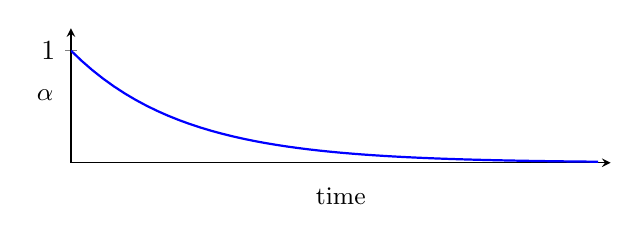
\begin{tikzpicture}
		\begin{axis}[
		%scale=0.6,
		ymax=1.2, ymin=0, xmin=0, xmax=3,samples=50, 
		ytick={1},
		axis lines=left, 
		xtick=\empty,
		yscale=0.3,
		ylabel style={rotate=-90},
		ylabel={\small $\alpha$},
		xlabel={\small time},
		%		every axis x label/.style={
		%			at={(ticklabel* cs:-0.5)},
		%			anchor=south,
		%		}
		every axis x label/.style={at={(current axis.south)},below=2mm},
		every axis y label/.style={at={(current axis.west)},left=1mm},
		]
		\addplot[blue, thick,domain=0:2.93] (x, 5^-x);
		%\addplot[red,  ultra thick] (x*x,x);
		\end{axis}
		\end{tikzpicture}
		\caption{Desired impact profile on $\alpha$ as a function of time}
		\label{fig:alphaTime}
	\end{center}
\end{figure}

%\subsubsection{Favoring }

\subsubsubsection{Penalizing velocity}

To also take velocity into account, we will consider the spatial length of the current movement vector $\b{\delta}$. First, we will want to ensure a responsive interface by fully discarding the past for very fast movements, i.e. some velocity threshold, but obviously not so low so as to be triggered by the inherent velocity of the noise. Also, we would like some sharp, but smooth transition in reaching this threshold, with profile as shown in figure \ref{fig:alphaVelocity}. We may capture such profile and threshold by a combined positive polynomial and cut-off function
$$\nu_n = \max \(0, 1- \lambda \norm{\b{\delta}}^2 \) $$ 
for some constant $\lambda$ determined by visual inspection.
\begin{figure}[!ht]
	\begin{center}
		\begin{tikzpicture}
		\begin{axis}[ymax=1.2, ymin=0, xmin=0, xmax=3,samples=50, 
		ytick={1},
		axis lines=left, 
		xtick=\empty,
		yscale=0.3,
		ylabel={\small $\alpha$},
		xlabel={\small velocity},
		ylabel style={rotate=-90},
		every axis x label/.style={at={(current axis.south)},below=2mm},
		every axis y label/.style={at={(current axis.west)},left=1mm},
		]
		\addplot[blue, thick] (x, 1 - 0.2 * x*x);
		\addplot[blue, ultra thick, ,domain=2.23:2.93] (x, 0);
		%\addplot[red,  ultra thick] (x*x,x);
		\end{axis}
		\end{tikzpicture}
		\caption{Desired impact profile on $\alpha$ as a function of velocity}
		\label{fig:alphaVelocity}
	\end{center}
\end{figure}

\subsubsubsection{Combined penalizations}

Incorporating the two penalizations in (\ref{eq:alphamSoothing}) gives the recurrence
\begin{eq}
%	\gamma_n
	\b{\tau_{n+1}} & = 
	\b{t_n} - \alpha_n \b{\delta}
	\\ & =
	\b{t_n} -   \pi_n \nu_n   \b{\delta}	 
	\\ & =
	\b{t_n} - \( \gamma^{-t} \) \( \max(0, 1- \lambda  \norm{\b{\delta}}^2) \) (\b{t_n} - \b{\tau_n})% \b{\delta} 
\end{eq}
which is the algorithm for ensuring a smooth transition  from on-screen to off-screen space, such that the user's sense of continuity is maximized.

To conclude, we will remark briefly on the expected behavior of this. First, the penalty imposed by time is assumed to be close to constant, since the frame rate of the tracker is approximately constant. Second, rapid navigations that exceed the velocity cut-off are assumed to be rare and constitute only a minor portion of all navigation. Hence, the general swiping speeds are not expected to fluctuate wildly, but rather increase or decrease in a relatively smooth manner. As such, the penalty imposed by velocity is also somewhat constant. This means that the weights do not fluctuate much within brief time periods, such that
$$\alpha_0 \approx \alpha_1 \approx \dots \approx \alpha_n $$
. If so, the recurrence will then resemble 
\begin{eq}
	\b{\tau_{n+1}} = \ &  (1 - \alpha) \b{t_n} + 
	\\
	&  \alpha (1 -\alpha) \b{t_{n-1}} + \dots +
	\\ 
	&  \alpha^{j}   (1 - \alpha ) \b{t_{n-j}} +  \dots +  
	\\
	&  \alpha^{n+1}  \b{\tau_0}   
\end{eq}
which is the \ti{exponential average} of past observations. This is the weighting between the present and past that is assumed intuitive  for stabilizing the input in general, but one that still ensures responsiveness by favoring the present for large velocities. 



%In addition, proper callibration was straightforward to confirm by visual inspecting, i.e. that the user moving the indedx finger freely in offscreen space was reflected in accurate and responsive projection onto the offscreen (visible as a cursor) .




